\begin{figure*}
    \centering
    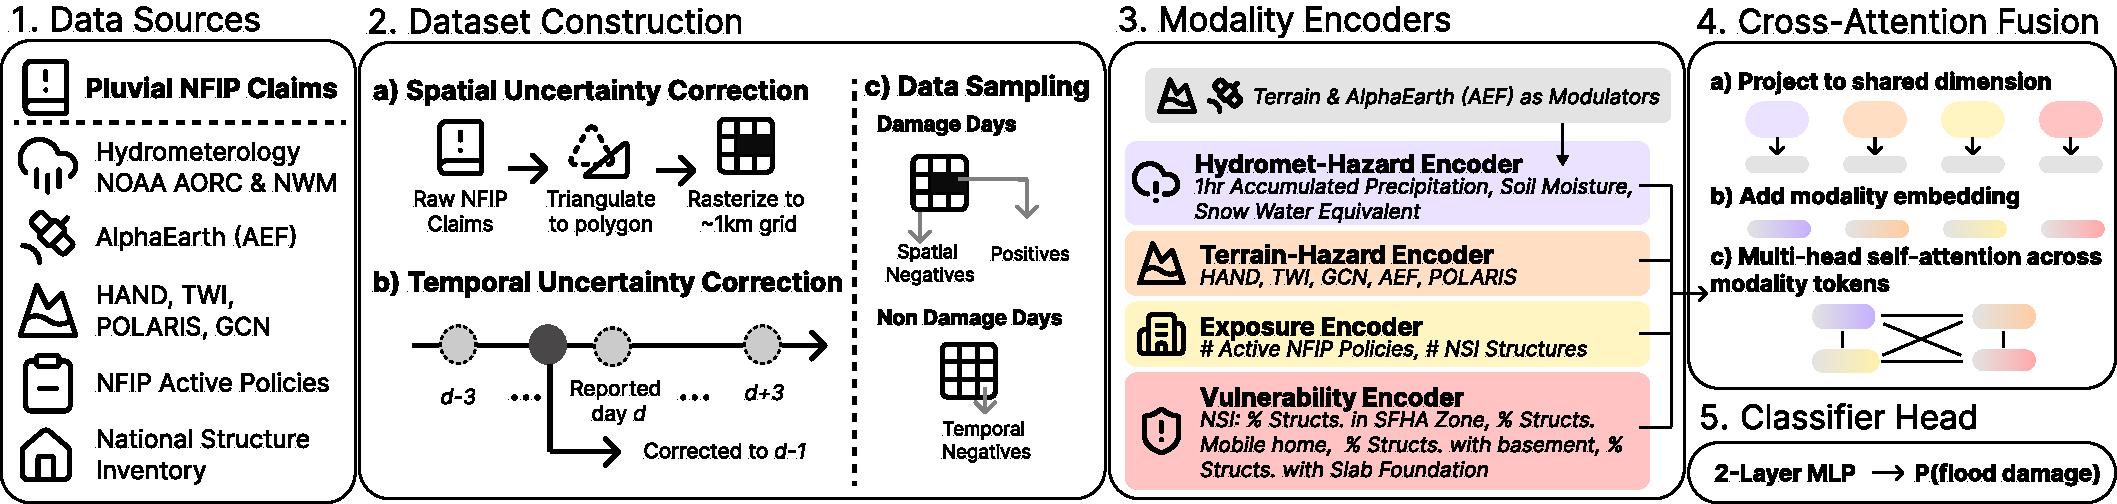
\includegraphics[width=\textwidth]{figs/Workflow.pdf}
    \caption{\textbf{DELUGE architecture.} DELUGE is a multimodal CNN-based model that integrates various data modalities, including meteorological, terrain-hazard, vulnerability, and exposure features, to predict pluvial flood damage at a daily and $\sim$1km resolution across the highest-claim regions of CONUS. The model consists of separate CNN branches for each modality, which are then fused together to produce the final damage prediction. The hydrometeorology branch is described in
 detail in Fig.~\ref{fig:modulators}.}
    \vspace{-0.15in}
    \label{fig:deluge_architecture}
\end{figure*}
Pluvial flooding is often a localized event with dynamics that depend strongly on local conditions such as topography, land use, and drainage infrastructure.
%
Although pluvial events, especially street-level events, may occur at sub-kilometer scales~\cite{lowe_urban_2020} beyond the resolution of our modeling, we provide the model with a larger \tsim$8\times8$\,km spatial context centered on each sample (a $7\times7$ pixel patch) for two reasons.

First, prior work has identified the spatial scale at which pluvial flooding develops~\cite{cristiano_spatial_2017,weiler_pluvial_2025}.
%
The effective extent varies across locations, but our \tsim$8\times8$\,km context covers the scale of pluvial flooding identified in the literature.
%
Second, pluvial flood events are often driven by convective storms~\cite{li_conterminous_2022} that deposit large amounts of precipitation in a localized area.
%
These extreme precipitation events are less reliably captured in the NOAA AORC archive~\cite{fall_analysis_2023}, and we expect their reported locations to carry variable spatial noise even with the latest observational and radar-based products.
%
A larger spatial context lets the model associate observed damage with the precipitation pattern in the surrounding area, which is more reliably recorded than the storm's exact center.
% with the spatial scale of pluvial flooding and associated hydrological process identified in the literature \cite{cristiano_spatial_2017}.
%
These considerations motivate DELUGE, the multimodal CNN-based model described in the following sections.
\vspace{-5pt}
  \subsection{Overview}
\label{sec:arch-overview}

We predict per-pixel binary pluvial flood insurance claims occurrence at $\sim$1.17~km resolution across the highest-claim regions of CONUS (\S\ref{ssec:study_region}) by fusing four modality branches (hydrometeorology, terrain, exposure, and vulnerability) into a per-pixel probability (Figure~\ref{fig:deluge_architecture}).
%
With respect to the standard triad in disaster risk modeling, the hydrometeorology and terrain branches capture the hazard, while the exposure and vulnerability branches capture exposure and vulnerability respectively.
%
Our target is the center pixel of a $7 \times 7$ patch (\tsim$8\times8$km) and all branches operate on this patch.
% Under the severe class imbalance of NFIP claims ($\sim$0.25\% positive, $\sim$1{,}800 events in $\sim$720K samples), we partition training, validation, and test cells via AEF-informed spatial clustering (Section~\ref{sec:arch-training}) to prevent geographic leakage.
\subsubsection{Supporting interpretability}
Predictive accuracy alone is insufficient for models intended to inform real-world flood-risk decisions.
%
Insurers and emergency managers must be able to inspect and justify a model's reasoning before acting on its outputs, especially under the high financial stakes of flood damage.
%
Prior work in deep-learning based flood and hydrological modeling has emphasized this same need for interpretability~\cite{taghizadeh_interpretable_2024, li_interpretable_2024, lee_improving_2024}.
%
We target this need at the architecture level, designing modulators (\S\ref{sec:arch-warp} and \ref{sec:arch-kernel}) whose hydrological response parameters are directly inspectable, a distinct goal from per-prediction interpretability.

We expose this interpretability via the hydrometeorology branch, the most important modality for prediction, where we develop two terrain and foundation model-conditioned modules that modulate the hydrometeorology signal along its two axes.
% \begin{itemize}[noitemsep, topsep=0pt, left=0pt, align=left]    
    % \item \emph{Value modulator} (Section~\ref{sec:arch-warp}), which learns a per-patch, per-channel monotonic warp of the hydrometeorology value range (value axis).
    % \item \emph{Temporal modulator} (Section~\ref{sec:arch-kernel}), which learns a per-patch mixed gamma-kernel hydrological response over the hydrometeorology lookback window (time axis); and
% \end{itemize}
First, the \emph{Value modulator} (Section~\ref{sec:arch-warp})  learns a per-patch, per-channel monotonic warp of the hydrometeorology value range (value axis) and then the \emph{Temporal modulator} (Section~\ref{sec:arch-kernel}), which learns a per-patch mixed gamma-kernel hydrological response over the hydrometeorology lookback window (time axis).
%
Both modules are terrain and foundation model-conditioned, so their parameters vary spatially as explicit model outputs (Fig.~\ref{fig:modulators}).
%
Conditioned on the local place characteristics, they answer two questions: which range of values in the hydrometeorology signal is most relevant to flood damage (\emph{Value Modulator}), and what temporal pattern of the hydrometeorology signal is most relevant to flood damage (\emph{Temporal Modulator}).

A similar module to our \emph{Value Modulator} was offered in \cite{taghizadeh_interpretable_2024} via Kolmogorov-Arnold Networks (KAN), but here we allow the model to learn location-specific warps that are conditioned on each local terrain and foundation model features.
%
This is a deliberate \emph{interpretability-by-design} choice rather than the more common path of pairing a flexible black-box encoder (ConvLSTM, Transformer) with post-hoc attribution (SHAP, integrated gradients, attention visualization)~\cite{rudin_stop_2019}, allowing us to inspect the model's reasoning directly from hydrologically meaningful, spatially explicit modulator parameters instead of generic feature importance scores.
% We prefer the by-design path for two reasons. \emph{Faithfulness}: the modulator parameters are not an approximation of the model dynamics but the computation itself.
% %
% \emph{Domain semantics}: kernel peak lag, decay timescale, fast/slow mode mixing, and value-warp breakpoints are hydrology vocabulary, readable directly without translation through generic feature-importance scores. 
% $\emph{Coupled inductive bias}: the parametric form does double duty as a regularizer in the signal-limited NFIP regime---a ConvLSTM-plus-attribution stack uses a high-capacity model that overfits sparse labels and then tries to attribute the overfit, whereas the modulator path uses a low-capacity, physics-shaped model that fits better \emph{and} reads directly. 
% As a corollary, the resulting per-cell parameter maps stand on their own as scientific artifacts, usable downstream by hydrologists independently of the predictive task.

% The outputs from the two modulators are then fused with the other branches and fed into a classifier head to produce the final per-pixel probability.
%
% Together they yield the first per-cell pluvial-flood hydrological-response and intensity-response maps for the United States. The maps' value is orthogonal to predictive PR-AUC: they are spatial-scientific artifacts derived directly from the learned weights.

% Throughout the architecture we favor parametric inductive bias over expressive black-box capacity. NFIP data is sparse, noisy in dating and geocoding, and concentrated in a small number of damage cells: the regime is signal-limited rather than capacity-limited. We document the resulting design ablations in Section~\ref{sec:arch-design}.

% The remainder of this section describes the inputs (Section~\ref{sec:arch-inputs}), the temporal kernel encoder (Section~\ref{sec:arch-kernel}), the per-cell value warp (Section~\ref{sec:arch-warp}), the other branches (Section~\ref{sec:arch-other}), cross-modal fusion (Section~\ref{sec:arch-fusion}), the classifier (Section~\ref{sec:arch-classifier}), and training (Section~\ref{sec:arch-training}).

\vspace{-7pt}
\subsection{Data Inputs}\label{ssec:arch-inputs}
% Each sample is a $7 \times 7$ pixel patch centered on the prediction pixel, plus higher-resolution modality features. Climate is sampled hourly over a $T = 73$~hour lookback ending at the prediction date $D$; terrain is static; vulnerability and AEF are annual (Table~\ref{tab:inputs}).

Predicting flood damages requires accounting for the three components of risk, hazard, exposure, and vulnerability, and we gather a comprehensive set of inputs to capture each.
%
\textbf{Hydrometeorological hazard} is drawn from hourly NOAA AORC accumulated precipitation~\cite{fall_analysis_2023} and 3-hourly NOAA National Water Model Retrospective volumetric soil moisture and snow water equivalent~\cite{cosgrove_noaas_2024}.
%
\textbf{Terrain hazard} combines the Topographic Wetness Index~\cite{hoylman_30m_2021}, Height Above Nearest Drainage~\cite{aws_copernicus_dem}, Global Curve Number under three antecedent runoff conditions~\cite{jaafar_gcn250_2019}, NLCD fractional impervious surface~\cite{usgs_annual_nlcd_2024}, and POLARIS soil properties (saturated hydraulic conductivity, clay percentage, and saturated water content)~\cite{chaney_polaris_2019}.
%
\textbf{Exposure and vulnerability} come from FIMA NFIP active policy counts and coverage~\cite{fema_nfip_policies_v2} and per-structure attributes from the USACE National Structure Inventory~\cite{usace_nsi_2022} (structure count, foundation types, mobile-home share, Special Flood Hazard Area [SFHA] membership, first-floor elevation statistics).
%
Finally, to complement these and to condition our modulators, we include 64-dimensional \textbf{Google AlphaEarth Foundation (AEF)} embeddings at 10\,m resolution~\cite{brown_alphaearth_2025}, which implicitly encode land cover and the built environment.
%
Per-source descriptions, exact variables used, and feature normalization details are deferred to the Appendix.

For each sample, a pixel-day tuple, we extract data for our modalities from the $7 \times 7$ pixel patch centered on the prediction pixel, bilinearly interpolating to match our $\sim$1.17~km resolution regular grid.
%
For inputs that are natively offered at a higher resolution, all sources except for the hydrometeorology and NFIP active policies, we extract the data at $56\times 56$ resolution.
%
For our hydrometeorology inputs, we extract a $T=73$-hour input window spanning Day~$D-2$ through Day~$D$ (inclusive).
%
The temporal modulator (\S\ref{sec:arch-kernel}) convolves this window with an $L=48$-hour kernel, and the temporal reduction selects a peak-response hour within Day~$D$.
%
The two are sized so that every reduction hour in Day~$D$ has its full $L=48$-hour kernel reach contained inside the $T=73$-hour input, requiring no padding.
%
We choose a 48-hour time window by considering the typical temporal dynamics of pluvial flooding, which can occur rapidly within hours of heavy rainfall, but also considering the need to capture antecedent conditions like soil moisture that can influence flood risk~\cite{bouwens2018towards,upreti2021comparison,james_precipitation_2024}.
%
A 48-hour kernel allows us to capture both the immediate impact of precipitation and the influence of prior hydrometeorological conditions, providing a comprehensive view of the factors contributing to pluvial flooding.
% (i.e. from $D-2$ to $D$ including the end points) to capture the temporal dynamics of pluvial flooding.
%
% We detail the source and shapes of each input in Table~\ref{tab:inputs}.

\begin{table*}[t]
\centering
\small
\setlength{\tabcolsep}{4pt}
\begin{tabular}{@{}p{0.18\linewidth}p{0.62\linewidth}c@{}}
\toprule
Modality & Source & Shape \\
\midrule
Hydrometeorology & Precipitation (NOAA AORC~\cite{fall_analysis_2023}); soil moisture and snow water equivalent (NWM v3~\cite{cosgrove_noaas_2024}) & $7 \times 7 \times 73 \times 3$ \\
Terrain & HAND~\cite{aws_copernicus_dem}, TWI~\cite{hoylman_30m_2021}, GCN (dry/avg/wet)~\cite{jaafar_gcn250_2019}, POLARIS ($K_{sat}$, clay, $\theta_s$)~\cite{chaney_polaris_2019} & $56 \times 56 \times 8$ \\
Foundation Model & AlphaEarth embeddings~\cite{brown_alphaearth_2025} & $56 \times 56 \times 64$ \\
Exposure & NSI building inventory~\cite{usace_nsi_2022}, NFIP active policies~\cite{fema_nfip_policies_v2} & $56 \times 56 \times 2$ \\
Vulnerability & NSI structural~\cite{usace_nsi_2022}, NFIP policy attributes~\cite{fema_nfip_policies_v2} & $56 \times 56 \times 10$ \\
\bottomrule
\end{tabular}\\[2pt]
\caption{DELUGE's input modalities and tensor shapes $(H \times W \times C)$. For hydrometeorology, the third axis is the $T=73$-step hourly window and the final dimension stacks the three channels; for other modalities the last axis is the feature-channel count.}
    \vspace{-0.15in}
\label{tab:inputs}
\end{table*}

% The three climate variables capture complementary mechanisms relevant to pluvial flooding: APCP is the proximate causal flux; SOIL\_M carries antecedent saturation state; SNEQV accounts for melt contributions. We omit NWM's accumulated underground runoff (UGDROFF)---it represents deep percolation to baseflow, the slowest hydrologic process in the dataset and more relevant to fluvial than pluvial flooding. In ablation it was redundant with SOIL\_M and offered no validation gain.
\subsection{Value Modulator}\label{sec:arch-warp}

Raw hydrometeorology values often span large ranges, and their flood-relevance is nonlinearly distributed across that range. 
%
For instance, a soil moisture measurement of $0.2~\mathrm{m^3\,m^{-3}}$ may be more relevant to pluvial flood dynamics in one location than in another.
%
Standard ML pipelines typically apply a global transformation (e.g.\ min-max standardization or a log transform) to the raw values, but we expect the value-relevance relationship to vary across locations, so such a one-size-fits-all transformation may miss this local variability.
%
This motivates our \emph{Value Modulator}, which learns a per-patch, per-channel transformation of the raw climate values, conditioned on the local terrain and foundation model features which we call a \emph{warp}.

\paragraph{Warp definition.}
For each hydrometeorology channel $v$ and patch $i$, the value modulator produces $K = 16$ width parameters $\{u_{v,i,k}\}_{k=1}^{K}$ and $K = 16$ height parameters $\{h_{v,i,k}\}_{k=1}^{K}$, each softmax-normalized so 
\[\sum_k u_{v,i,k} = \sum_k h_{v,i,k} = 1\]
%
We choose $K=16$ as a balance between expressivity and simplicity, finding 16 control points sufficient to capture the value-relevance relationship.
%
These control points define cumulative breakpoints on the input and output axes, so that $X_{v,i,k} \;=\; \sum_{j=1}^{k} u_{v,i,j}$ and $Y_{v,i,k} \;=\; \sum_{j=1}^{k} h_{v,i,j}$,with $X_{v,i,0} = Y_{v,i,0} = 0$ and $X_{v,i,K} = Y_{v,i,K} = 1$. 
%
The warp $\phi_{v,i} : [0, 1] \to [0, 1]$ is then a monotonic piecewise-linear map satisfying $\phi_{v,i}(X_{v,i,k}) = Y_{v,i,k}$, with slope $m_{v,i,k} = h_{v,i,k} / u_{v,i,k}$ inside the $k$-th segment.
%
We define the warp, $\phi_{v,i}$, for each $\tilde{x}\in [X_{v,i,k-1},\, X_{v,i,k}]$ as 
\[\phi_{v,i}(\tilde{x}) \;=\; Y_{v,i,k-1} + m_{v,i,k}\,(\tilde{x} - X_{v,i,k-1})\]
%
% \begin{equation}
%     \phi_{v,i}(\tilde{x}) \;=\; Y_{v,i,k-1} + \frac{h_{v,i,k}}{u_{v,i,k}}\,(\tilde{x} - X_{v,i,k-1}) 
% \end{equation}
% Softmax normalization on both $\{u\}$ and $\{h\}$ guarantees monotonicity and a fixed $[0,1] \to [0,1]$ domain/range without further constraints.

\paragraph{Application.}
Each raw input $x_v[t, i]$ is first min-max normalized to $\tilde{x}_v[t, i] \in [0, 1]$ using channel-specific bounds, then the warp is applied to produce the warped value.
\[\tilde{x}^{\,\prime}_v[t, i] \;=\; \phi_{v,i}\!\left(\tilde{x}_v[t, i]\right)\]
% \begin{equation}
%     \tilde{x}^{\,\prime}_v[t, i] \;=\; \phi_{v,i}\!\left(\tilde{x}_v[t, i]\right)
% \end{equation}
The warp $\phi_{v,i}$ varies per channel and per patch but is \emph{shared across time steps} within the input window, so a single learned warp reshapes every channel $v$ at patch $i$ identically. The warped sequence $\tilde{x}^{\,\prime}_v[t, i]$ then forms the input to the temporal modulator (\S\ref{sec:arch-kernel}).

\paragraph{Per-patch terrain and foundation-model conditioning.}
The $2K \cdot V$ warp parameters per patch are produced by a terrain- and foundation-model-conditioned module \textsc{value\_modulation}, a single convolution layer on the stacked terrain and AEF features followed by a two-layer MLP.
%
We zero-initialize the weights and biases of this module's final layer, so the softmax over $u_{v,i,k}$ and $h_{v,i,k}$ yields uniform widths and heights at the start of training. The initial warp is therefore the identity map $\phi_{v,i}(\tilde{x}) = \tilde{x}$, and training departs from this identity as each patch's terrain and AEF context pushes its breakpoints apart.
\begin{figure*}[ht]
    \centering
    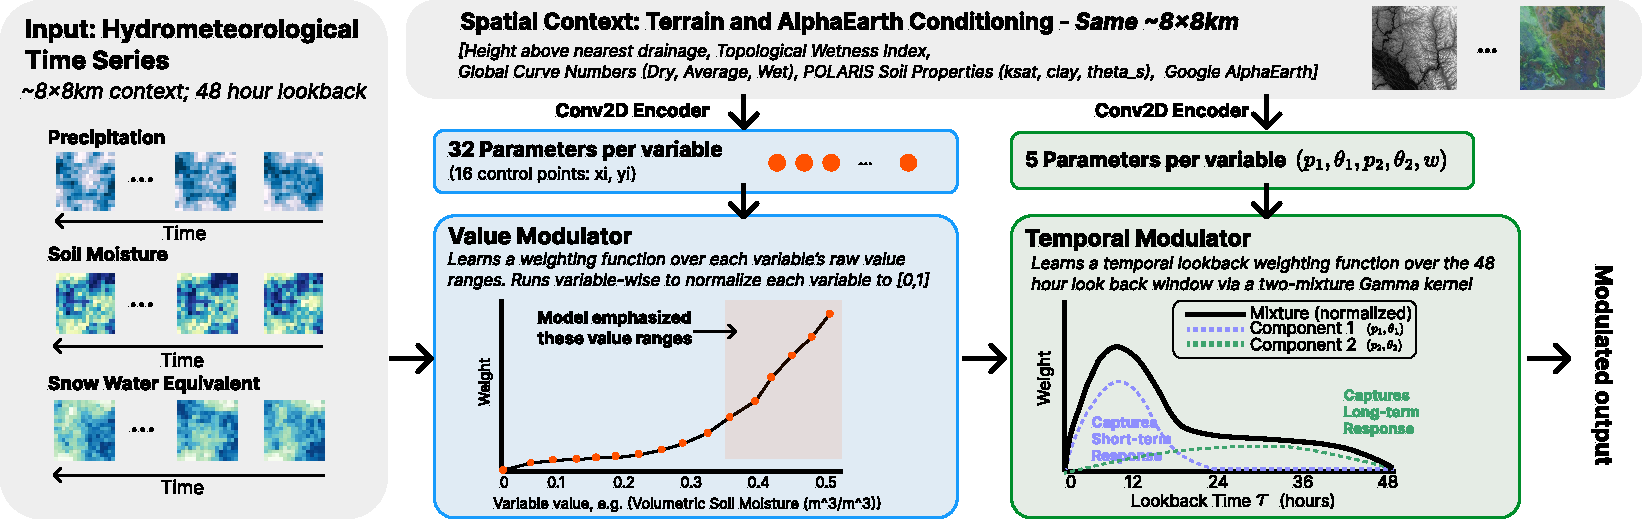
\includegraphics[width=\textwidth]{figs/Modulators.pdf}
    \caption{The two terrain- and AEF-conditioned modulators acting on the hydrometeorology branch. The \textbf{Value Modulator} (\S\ref{sec:arch-warp}) applies a per-channel, per-patch piecewise-linear warp $\phi_{v,i}:[0,1]\!\to\![0,1]$ to each min-max normalized input, reshaping the response curve along the value axis. The \textbf{Temporal Modulator} (\S\ref{sec:arch-kernel}) then convolves the warped sequence with a per-channel gamma-kernel mixture $k_v(\tau)$,
    integrating the $T$-hour lookback along the time axis. Each modulator has its own conditioning network (ConvBlock + MLP) over the stacked terrain and AlphaEarth Foundation features, making the learned warp shapes and kernel peaks/decay timescales directly interpretable per patch.}\label{fig:modulators}
    \vspace{-0.15in}
\end{figure*}
\subsection{Temporal Modulator}
\label{sec:arch-kernel}


% Standard temporal encoders (ConvLSTM, TCN, Transformer) compress this window through opaque operations, foreclosing extraction of the response function the model discovers per cell. We instead use a parametric gamma-kernel module whose learned per-cell parameters admit a direct hydrological interpretation.

\paragraph{Gamma kernels and two-component mixture.}
For each channel $v$ and lag $\tau \in \{0, \ldots, L{-}1\}$ with kernel lookback $L = 48$, a single gamma kernel parameterized by peak lag $p$ and timescale $\theta$ is the discretized, normalized Gamma$(\alpha, \theta)$ density: 
\[k(\tau; p, \theta) \;=\; \frac{\tau^{\alpha - 1}\, e^{-\tau/\theta}}{\sum_{\tau'=0}^{L-1} (\tau')^{\alpha - 1}\, e^{-\tau'/\theta}},\] where $\alpha = \tfrac{p}{\theta} + 1$.
% \begin{equation}
%     k(\tau; p, \theta) \;=\; \frac{\tau^{\alpha - 1}\, e^{-\tau/\theta}}{\sum_{\tau'=0}^{L-1} (\tau')^{\alpha - 1}\, e^{-\tau'/\theta}}, \quad \alpha = \tfrac{p}{\theta} + 1.
% \end{equation}
We reparameterize the shape via $\alpha = p/\theta + 1$ so that the kernel's peak lag is exactly $p$ (the mode of Gamma$(\alpha, \theta)$ lies at $(\alpha - 1)\theta = p$), making the two learned parameters $(p, \theta)$ directly interpretable: $p$ is the peak response time in hours and $\theta$ is the decay timescale in hours. 
%
% In practice, we evaluate $k(\tau)$ as a softmax over $(\alpha - 1)\log(\tau + \varepsilon) - \tau/\theta$ for numerical stability. 
%
The gamma is chosen here as a flexible, two-parameter kernel often used in hydrology to model rainfall-runoff response~\cite{nash_systematic_1959}.
% ; with its single mode and exponential tail, it spans temporal patterns from sharply peaked and fast-decaying to broad and slowly decaying.
% The gamma form arises as the impulse response of a Nash cascade of linear reservoirs~\fix{cite}, a strong inductive bias for rainfall-runoff temporal patterns.

To capture varied temporal patterns, we adopt a per-channel convex mixture of two gammas with the same functional form but different parameters for the precipitation channel.
%
Here, we parameterize a convex mixture of two gamma, weighted by a learnt mixing weight $w_v$: $k_v(\tau) \;=\; w_v\, k(\tau; p^{\text{1}}_v, \theta^{\text{1}}_v) \;+\; (1 - w_v)\, k(\tau; p^{\text{2}}_v, \theta^{\text{2}}_v)$.
% \begin{equation}
%     k_v(\tau) \;=\; w_v\, k(\tau; p^{\text{1}}_v, \theta^{\text{1}}_v) \;+\; (1 - w_v)\, k(\tau; p^{\text{2}}_v, \theta^{\text{2}}_v),
% \end{equation}
%
For soil moisture and snow water equivalent, we employ a single gamma.
%
% with the ordering $p^{\text{s}}_v = p^{\text{f}}_v + (L - p^{\text{f}}_v)\,\rho_v$ enforced, where $\rho_v \in (0, 1)$ is a sigmoid-bounded learned offset; this guarantees $p^{\text{s}}_v > p^{\text{f}}_v$ and prevents the fast and slow modes from being swappable across training runs. 
% All other kernel parameters are sigmoid-bounded: $p_v \in [0.5, L]$, $\theta \in [0.5, L]$~hours, $w \in (0, 1)$. 
% 
% We bound $p_v$ below with 0.5 to avoid numerical instability.
%
In all, each channel's temporal response kernel is parameterized by five (precipitation) or two (rest) parameters, totaling  kernel parameters per patch.

\paragraph{Per-patch terrain conditioning.}
The \textsc{temporal\_modulation} module is structurally analogous to \textsc{value\_modulation}, producing the 9 kernel parameters per patch from the stacked terrain and AEF features.
% The kernel parameters are produced per cell by a AEF\&terrain-conditioned module: a single $3 \times 3$ ConvBlock ($C_t \to 64$) over the stacked terrain and AEF features $\mathbf{t}$ followed by global average pooling and a two-layer MLP to produce the 15 parameters per sample.
%
% The ConvBlock preserves the terrain texture (slope variance, imperviousness patchiness) that pure pooling would discard. 
%
The final linear layer is zero-initialized in weight, with bias chosen so each cell decodes the same hydrologically reasonable kernel at step 0 ($p^{\text{1}} \approx 3$h, $p^{\text{2}} \approx 24$h, $\theta^{\text{1}} \approx 3$h, $\theta^{\text{2}} \approx 12$h, $w \approx 0.5$); training then pushes per-patch parameters apart based on each patch's characteristics.

\paragraph{Causal convolution}
Let $i$ be one of the pixels within the $7 \times 7$ patch, and let $x_v[t, i]$ denote the value of hydrometeorology channel $v$ at time $t$ and pixel $i$ within the $T$-hour input window. The kernel $k_v$ is then convolved causally with the input sequence to produce the response at pixel $i$: \[r_v[t, i] \;=\; \sum_{\tau=0}^{L-1} k_v(\tau)\, x_v[t - \tau,\, i].\]
The kernel is shared across all pixels within the patch.
%
\paragraph{Temporal reduction}
The temporal axis is collapsed by selecting one time step $t'$ per pixel, the moment of peak accumulated precipitation \emph{response} within Day~$D$: $t'(i) = \operatorname*{argmax}_{t \in \text{Day D}} r_{\text{precip}}[t, i]$. 
%
We reduce this via, $r_{\text{reduced}}[v, i] = r_v[t'(i), i]$.
%
All channels are read at the same $t'$, yielding a temporally-coherent Day-$D$ snapshot.
%
We expect this to summarize the hydrometeorological state at the moment of peak precipitation impact, appropriately weighing the lookback hours according to the learned kernel.
%
Finally, a linear $1 \times 1$ convolution lifts the per-pixel $V$-dimensional reduced response to a 32D feature space for fusion with the other modalities.
% \begin{equation}
%     \mathbf{h} \;=\; \mathrm{Dropout}\!\left(\mathrm{LeakyReLU}(\mathbf{W}\, r_{\text{red}} + \mathbf{b})\right), \quad \mathbf{h} \in \mathbb{R}^{B \times 16 \times H \times W}.
% \end{equation}
% We use a linear projection rather than a nonlinear bottleneck: nonlinear heads back-pressure the kernel parameters during training (Section~\ref{sec:arch-design}), eroding the interpretability of the learned $(p, \theta)$ maps. The kernel encoder itself uses $\sim$80 parameters; the dominant cost is the terrain conditioner at $\sim$15K parameters---roughly one-quarter of an equivalent ConvLSTM encoder.

\vspace{-3pt}
\subsection{Other Components}
\paragraph{Modality Encoders.}

The remaining three modalities are processed by lightweight convolutional encoders, all operating on the same \tsim$8\times8$\,km patch.
%
The NSI building-inventory and structural fields are native to the $56 \times 56$ grid, while the NFIP active-policy and policy-attribute fields are native to the $7 \times 7$ grid and are bilinearly upsampled to $56 \times 56$, so the \emph{Terrain-Hazard}, \emph{Exposure}, and \emph{Vulnerability} encoders all operate at a common $56 \times 56$ resolution.
%
Each encoder maps its input through strided convolutional blocks that downsample to $7 \times 7$, producing 16, 8, and 8 channels respectively.
%
All encoders use $3 \times 3$ convolutions, leaky-ReLU activations, and batch normalization~\cite{ioffe_batch_2015}.

\paragraph{Cross-Modal Fusion.}

At each of the $7 \times 7$ spatial positions, the four modality feature vectors form a set of four tokens.
%
Each token is linearly projected to $d_{\text{model}} = 32$ by a $1 \times 1$ convolution and summed with a learnable modality-type embedding that identifies its source modality.
%
We fuse the tokens with a single Transformer encoder layer~\cite{vaswani_attention_2017}, applying 4-head self-attention and a position-wise feed-forward network, each wrapped in a residual connection and layer normalization, so that every modality attends to the others before fusion.
%
The fused representation $f$ is read out at the center pixel to align with the per-pixel prediction target.

\paragraph{Classifier.}
\label{sec:arch-classifier}

The center-pixel feature vector $f \in \mathbb{R}^{d_{\text{model}}}$ is mapped to a claim probability by an MLP classification head with a single hidden layer.
%
The hidden layer applies layer normalization and a GELU nonlinearity~\cite{hendrycks_gaussian_2016}, and a final linear layer with a sigmoid activation produces the per-pixel probability $\hat{y} \in [0,1]$.

\subsection{Training}
\label{sec:arch-training}

\paragraph{Spatial Holdout Split.}
To prevent spatial leakage, we partition the 100 grid cells (\S\ref{ssec:study_region}) into train and test sets at the 75\,km cell level rather than at the pixel level.
%
We use a spatially blocked split of grid cells, so the model is evaluated on held-out geographic regions rather than on held-out samples from the same regions.
%
Because our 100 grid cells span the diverse hydroclimatic regions of CONUS, across which flood dynamics are known to vary significantly~\cite{brunner_spatial_2020}, evaluating on spatially held-out cells tests whether DELUGE generalizes across this wide range of flood dynamics rather than to new samples from cells it has already seen.
\paragraph{Loss.} We use focal loss~\cite{lin_focal_2020} with $\alpha = 0.5$, $\gamma = 2$, weighted per sample by our claim polygon area based confidence score $c$ (\S\ref{ssec:dataset_construction}).
% 
This choice is primarily motivated by the extreme class imbalance and to de-emphasize the easy negative samples, which are abundant in the dataset and can overwhelm the learning signal from the more informative positive samples.
%
% We empirically found focal loss to outperform binary cross-entropy, likely because it better handles the extreme class imbalance and suppresses easy minority class samples.

In addition to the main loss on the predicted flood probability, we add a smoothness penalty on the Value Modulator's parameters (\S\ref{sec:arch-warp}):
\[\mathcal{L}_{\text{smooth}}=\sum_{v} \frac{1}{K-1} \sum_{k=1}^{K-1} \left[(u_{v,k+1} - u_{v,k})^2 + (h_{v,k+1} - h_{v,k})^2\right]\]
% \begin{equation}
%     \mathcal{L}_{\text{smooth}}=\sum_{v} \frac{1}{K-1} \sum_{k=1}^{K-1} \left[(u_{v,k+1} - u_{v,k})^2 + (h_{v,k+1} - h_{v,k})^2\right]
% \end{equation}
%
The penalty encourages adjacent widths and adjacent heights to vary smoothly across segments, biasing the learned warp toward a smooth function.
% The softmax constraints already enforce monotonicity and the $[0, 1] \to [0, 1]$ boundary conditions; the smoothness term is the additional inductive bias that keeps the learned warps human-readable.
% 
In all, we optimize for the weighted sum of the focal loss and the smoothness penalty:
$\mathcal{L} \;=\; \mathcal{L}_{\text{focal}} + \lambda\cdot\mathcal{L}_{\text{smooth}}$ with $\lambda = 0.1$.
% \begin{equation}
% \mathcal{L} \;=\; \mathcal{L}_{\text{focal}} + \lambda\cdot\mathcal{L}_{\text{smooth}}, \quad \lambda = 0.1
% \end{equation}
We apply the AdamW optimizer~\cite{loshchilov_decoupled_2019} with a cosine learning-rate schedule and linear warmup.


% \noindent\textbf{Class imbalance.} Given the $\sim$0.25\% natural positive rate, a \emph{BalancedPixelSampler} undersamples negatives at the dataset level to a 10\% positive batch rate; each positive is seen once per epoch.

%
% The per-cell random split is a compromise that allows the model to learn generalizable flood dynamics while still being evaluated on held-out geographic regions.
% and we found it to yield more stable training and validation performance than full geographic blocking.
% ; the per-cell random split preserves geographic diversity in both train and test while still preventing within-cell leakage.

% Train, validation, and test grid cells are partitioned by clustering grid cells in AlphaEarth Foundation embedding space (which captures land-cover, urbanization, and surface-hydrology context), then assigning whole clusters to a single split. This ensures hydrologically-similar cells are not split across train and test, preventing geographic leakage stronger than naive random or latitude/longitude blocking would catch.
% \paragraph{Optimization.} 
%
% Training was done over 20 epochs.
% , bfloat16 mixed precision, and gradient clipping at $\|\mathbf{g}\| \le 1.0$.

% \subsection{Architectural Design Choices}
% \label{sec:arch-design}
%
% We justify five non-obvious choices via controlled ablations. Each alternative we tested gained on training but degraded validation PR-AUC, consistent with the signal-limited regime.
%
% \noindent\textbf{Parametric kernel over learned recurrence.} A ConvLSTM encoder matches the kernel encoder's validation PR-AUC at $\sim$4$\times$ the parameter count and produces no interpretable per-cell artifact. The gamma-kernel inductive bias absorbs the role the ConvLSTM's extra capacity played in memorizing training data.
%
% \noindent\textbf{Linear head over nonlinear bottleneck.} A two-layer nonlinear head increased train PR-AUC but degraded validation: the kernel parameters drifted to support the head's preferred multiplicative compositions rather than reflecting per-cell response timescales.
%
% \noindent\textbf{APCP-anchored Day-$D$ reduction over joint argmax.} A joint sum-over-channels argmax was empirically APCP-amplitude-dominated in any case; explicit anchoring is more honest and yields clearer per-cell maps.
%
% \noindent\textbf{Center-pixel readout over learned spatial attention.} The prediction target is the center pixel and upstream $3 \times 3$ convolutions already mix neighborhood signal into it; learned spatial attention was a redundant capacity layer.
%
% \noindent\textbf{ConvBlock-MLP conditioner over pure MLP.} A pool-first MLP conditioner discarded terrain texture and caused per-cell warp and kernel parameters to regress toward the mean on held-out cells; one ConvBlock preserves texture without the overfit risk of deeper conv stacks.
